% Created by tikzDevice version 0.10.1 on 2016-09-01 14:35:46
% !TEX encoding = UTF-8 Unicode
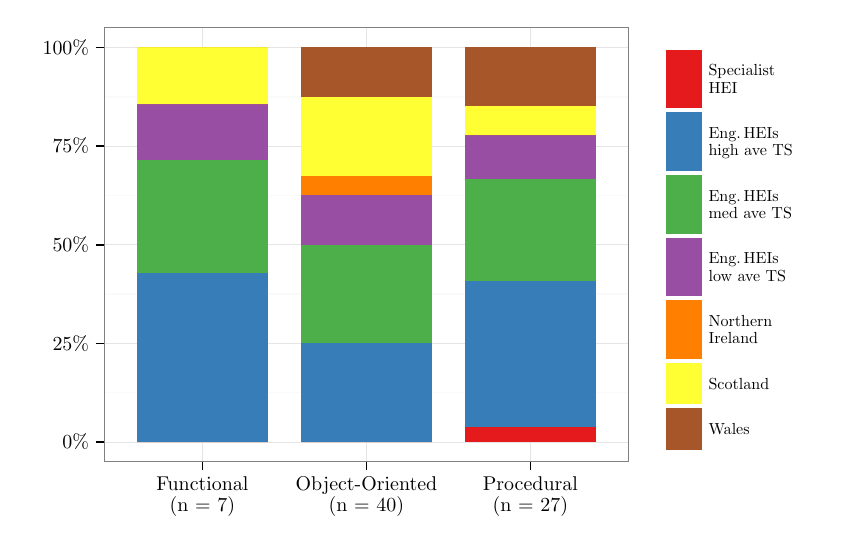
\begin{tikzpicture}[x=1pt,y=1pt]
\definecolor{fillColor}{RGB}{255,255,255}
\path[use as bounding box,fill=fillColor,fill opacity=0.00] (0,0) rectangle (289.08,180.67);
\begin{scope}
\path[clip] (  0.00,  0.00) rectangle (289.08,180.67);
\definecolor{drawColor}{RGB}{255,255,255}
\definecolor{fillColor}{RGB}{255,255,255}

\path[draw=drawColor,line width= 0.6pt,line join=round,line cap=round,fill=fillColor] (  0.00, -0.00) rectangle (289.08,180.67);
\end{scope}
\begin{scope}
\path[clip] ( 27.58, 23.83) rectangle (217.21,180.67);
\definecolor{fillColor}{RGB}{255,255,255}

\path[fill=fillColor] ( 27.58, 23.83) rectangle (217.21,180.67);
\definecolor{drawColor}{gray}{0.98}

\path[draw=drawColor,line width= 0.6pt,line join=round] ( 27.58, 48.78) --
	(217.21, 48.78);

\path[draw=drawColor,line width= 0.6pt,line join=round] ( 27.58, 84.43) --
	(217.21, 84.43);

\path[draw=drawColor,line width= 0.6pt,line join=round] ( 27.58,120.07) --
	(217.21,120.07);

\path[draw=drawColor,line width= 0.6pt,line join=round] ( 27.58,155.72) --
	(217.21,155.72);
\definecolor{drawColor}{gray}{0.90}

\path[draw=drawColor,line width= 0.2pt,line join=round] ( 27.58, 30.95) --
	(217.21, 30.95);

\path[draw=drawColor,line width= 0.2pt,line join=round] ( 27.58, 66.60) --
	(217.21, 66.60);

\path[draw=drawColor,line width= 0.2pt,line join=round] ( 27.58,102.25) --
	(217.21,102.25);

\path[draw=drawColor,line width= 0.2pt,line join=round] ( 27.58,137.90) --
	(217.21,137.90);

\path[draw=drawColor,line width= 0.2pt,line join=round] ( 27.58,173.55) --
	(217.21,173.55);

\path[draw=drawColor,line width= 0.2pt,line join=round] ( 63.13, 23.83) --
	( 63.13,180.67);

\path[draw=drawColor,line width= 0.2pt,line join=round] (122.39, 23.83) --
	(122.39,180.67);

\path[draw=drawColor,line width= 0.2pt,line join=round] (181.65, 23.83) --
	(181.65,180.67);
\definecolor{fillColor}{RGB}{228,26,28}

\path[fill=fillColor] ( 39.43, 30.95) rectangle ( 86.84, 30.95);
\definecolor{fillColor}{RGB}{55,126,184}

\path[fill=fillColor] ( 39.43, 30.95) rectangle ( 86.84, 92.07);
\definecolor{fillColor}{RGB}{77,175,74}

\path[fill=fillColor] ( 39.43, 92.07) rectangle ( 86.84,132.81);
\definecolor{fillColor}{RGB}{152,78,163}

\path[fill=fillColor] ( 39.43,132.81) rectangle ( 86.84,153.18);
\definecolor{fillColor}{RGB}{255,127,0}

\path[fill=fillColor] ( 39.43,153.18) rectangle ( 86.84,153.18);
\definecolor{fillColor}{RGB}{255,255,51}

\path[fill=fillColor] ( 39.43,153.18) rectangle ( 86.84,173.55);
\definecolor{fillColor}{RGB}{166,86,40}

\path[fill=fillColor] ( 39.43,173.55) rectangle ( 86.84,173.55);
\definecolor{fillColor}{RGB}{228,26,28}

\path[fill=fillColor] ( 98.69, 30.95) rectangle (146.10, 30.95);
\definecolor{fillColor}{RGB}{55,126,184}

\path[fill=fillColor] ( 98.69, 30.95) rectangle (146.10, 66.60);
\definecolor{fillColor}{RGB}{77,175,74}

\path[fill=fillColor] ( 98.69, 66.60) rectangle (146.10,102.25);
\definecolor{fillColor}{RGB}{152,78,163}

\path[fill=fillColor] ( 98.69,102.25) rectangle (146.10,120.07);
\definecolor{fillColor}{RGB}{255,127,0}

\path[fill=fillColor] ( 98.69,120.07) rectangle (146.10,127.20);
\definecolor{fillColor}{RGB}{255,255,51}

\path[fill=fillColor] ( 98.69,127.20) rectangle (146.10,155.72);
\definecolor{fillColor}{RGB}{166,86,40}

\path[fill=fillColor] ( 98.69,155.72) rectangle (146.10,173.55);
\definecolor{fillColor}{RGB}{228,26,28}

\path[fill=fillColor] (157.95, 30.95) rectangle (205.35, 36.24);
\definecolor{fillColor}{RGB}{55,126,184}

\path[fill=fillColor] (157.95, 36.24) rectangle (205.35, 89.05);
\definecolor{fillColor}{RGB}{77,175,74}

\path[fill=fillColor] (157.95, 89.05) rectangle (205.35,126.02);
\definecolor{fillColor}{RGB}{152,78,163}

\path[fill=fillColor] (157.95,126.02) rectangle (205.35,141.86);
\definecolor{fillColor}{RGB}{255,127,0}

\path[fill=fillColor] (157.95,141.86) rectangle (205.35,141.86);
\definecolor{fillColor}{RGB}{255,255,51}

\path[fill=fillColor] (157.95,141.86) rectangle (205.35,152.42);
\definecolor{fillColor}{RGB}{166,86,40}

\path[fill=fillColor] (157.95,152.42) rectangle (205.35,173.55);
\definecolor{drawColor}{gray}{0.50}

\path[draw=drawColor,line width= 0.6pt,line join=round,line cap=round] ( 27.58, 23.83) rectangle (217.21,180.67);
\end{scope}
\begin{scope}
\path[clip] (  0.00,  0.00) rectangle (289.08,180.67);
\definecolor{drawColor}{RGB}{0,0,0}

\node[text=drawColor,anchor=base east,inner sep=0pt, outer sep=0pt, scale=  0.72] at ( 22.18, 28.48) {0\%};

\node[text=drawColor,anchor=base east,inner sep=0pt, outer sep=0pt, scale=  0.72] at ( 22.18, 64.12) {25\%};

\node[text=drawColor,anchor=base east,inner sep=0pt, outer sep=0pt, scale=  0.72] at ( 22.18, 99.77) {50\%};

\node[text=drawColor,anchor=base east,inner sep=0pt, outer sep=0pt, scale=  0.72] at ( 22.18,135.42) {75\%};

\node[text=drawColor,anchor=base east,inner sep=0pt, outer sep=0pt, scale=  0.72] at ( 22.18,171.07) {100\%};
\end{scope}
\begin{scope}
\path[clip] (  0.00,  0.00) rectangle (289.08,180.67);
\definecolor{drawColor}{RGB}{0,0,0}

\path[draw=drawColor,line width= 0.6pt,line join=round] ( 24.58, 30.95) --
	( 27.58, 30.95);

\path[draw=drawColor,line width= 0.6pt,line join=round] ( 24.58, 66.60) --
	( 27.58, 66.60);

\path[draw=drawColor,line width= 0.6pt,line join=round] ( 24.58,102.25) --
	( 27.58,102.25);

\path[draw=drawColor,line width= 0.6pt,line join=round] ( 24.58,137.90) --
	( 27.58,137.90);

\path[draw=drawColor,line width= 0.6pt,line join=round] ( 24.58,173.55) --
	( 27.58,173.55);
\end{scope}
\begin{scope}
\path[clip] (  0.00,  0.00) rectangle (289.08,180.67);
\definecolor{drawColor}{RGB}{0,0,0}

\path[draw=drawColor,line width= 0.6pt,line join=round] ( 63.13, 20.83) --
	( 63.13, 23.83);

\path[draw=drawColor,line width= 0.6pt,line join=round] (122.39, 20.83) --
	(122.39, 23.83);

\path[draw=drawColor,line width= 0.6pt,line join=round] (181.65, 20.83) --
	(181.65, 23.83);
\end{scope}
\begin{scope}
\path[clip] (  0.00,  0.00) rectangle (289.08,180.67);
\definecolor{drawColor}{RGB}{0,0,0}

\node[text=drawColor,anchor=base,inner sep=0pt, outer sep=0pt, scale=  0.72] at ( 63.13, 13.47) {Functional};

\node[text=drawColor,anchor=base,inner sep=0pt, outer sep=0pt, scale=  0.72] at ( 63.13,  5.69) {(n = 7)};

\node[text=drawColor,anchor=base,inner sep=0pt, outer sep=0pt, scale=  0.72] at (122.39, 13.47) {Object-Oriented};

\node[text=drawColor,anchor=base,inner sep=0pt, outer sep=0pt, scale=  0.72] at (122.39,  5.69) {(n = 40)};

\node[text=drawColor,anchor=base,inner sep=0pt, outer sep=0pt, scale=  0.72] at (181.65, 13.47) {Procedural};

\node[text=drawColor,anchor=base,inner sep=0pt, outer sep=0pt, scale=  0.72] at (181.65,  5.69) {(n = 27)};
\end{scope}
\begin{scope}
\path[clip] (  0.00,  0.00) rectangle (289.08,180.67);
\definecolor{fillColor}{RGB}{255,255,255}

\path[fill=fillColor] (225.74, 23.19) rectangle (280.54,181.31);
\end{scope}
\begin{scope}
\path[clip] (  0.00,  0.00) rectangle (289.08,180.67);
\definecolor{fillColor}{RGB}{228,26,28}

\path[fill=fillColor] (230.72,151.51) rectangle (243.53,172.71);
\end{scope}
\begin{scope}
\path[clip] (  0.00,  0.00) rectangle (289.08,180.67);
\definecolor{fillColor}{RGB}{55,126,184}

\path[fill=fillColor] (230.72,128.88) rectangle (243.53,150.08);
\end{scope}
\begin{scope}
\path[clip] (  0.00,  0.00) rectangle (289.08,180.67);
\definecolor{fillColor}{RGB}{77,175,74}

\path[fill=fillColor] (230.72,106.25) rectangle (243.53,127.46);
\end{scope}
\begin{scope}
\path[clip] (  0.00,  0.00) rectangle (289.08,180.67);
\definecolor{fillColor}{RGB}{152,78,163}

\path[fill=fillColor] (230.72, 83.62) rectangle (243.53,104.83);
\end{scope}
\begin{scope}
\path[clip] (  0.00,  0.00) rectangle (289.08,180.67);
\definecolor{fillColor}{RGB}{255,127,0}

\path[fill=fillColor] (230.72, 60.99) rectangle (243.53, 82.20);
\end{scope}
\begin{scope}
\path[clip] (  0.00,  0.00) rectangle (289.08,180.67);
\definecolor{fillColor}{RGB}{255,255,51}

\path[fill=fillColor] (230.72, 44.58) rectangle (243.53, 59.57);
\end{scope}
\begin{scope}
\path[clip] (  0.00,  0.00) rectangle (289.08,180.67);
\definecolor{fillColor}{RGB}{166,86,40}

\path[fill=fillColor] (230.72, 28.17) rectangle (243.53, 43.16);
\end{scope}
\begin{scope}
\path[clip] (  0.00,  0.00) rectangle (289.08,180.67);
\definecolor{drawColor}{RGB}{0,0,0}

\node[text=drawColor,anchor=base west,inner sep=0pt, outer sep=0pt, scale=  0.58] at (246.04,169.46) {};

\node[text=drawColor,anchor=base west,inner sep=0pt, outer sep=0pt, scale=  0.58] at (246.04,163.24) {Specialist};

\node[text=drawColor,anchor=base west,inner sep=0pt, outer sep=0pt, scale=  0.58] at (246.04,157.02) {HEI};

\node[text=drawColor,anchor=base west,inner sep=0pt, outer sep=0pt, scale=  0.58] at (246.04,150.80) {};
\end{scope}
\begin{scope}
\path[clip] (  0.00,  0.00) rectangle (289.08,180.67);
\definecolor{drawColor}{RGB}{0,0,0}

\node[text=drawColor,anchor=base west,inner sep=0pt, outer sep=0pt, scale=  0.58] at (246.04,146.83) {};

\node[text=drawColor,anchor=base west,inner sep=0pt, outer sep=0pt, scale=  0.58] at (246.04,140.61) {Eng.\,HEIs};

\node[text=drawColor,anchor=base west,inner sep=0pt, outer sep=0pt, scale=  0.58] at (246.04,134.39) {high ave TS};

\node[text=drawColor,anchor=base west,inner sep=0pt, outer sep=0pt, scale=  0.58] at (246.04,128.17) {};
\end{scope}
\begin{scope}
\path[clip] (  0.00,  0.00) rectangle (289.08,180.67);
\definecolor{drawColor}{RGB}{0,0,0}

\node[text=drawColor,anchor=base west,inner sep=0pt, outer sep=0pt, scale=  0.58] at (246.04,124.20) {};

\node[text=drawColor,anchor=base west,inner sep=0pt, outer sep=0pt, scale=  0.58] at (246.04,117.98) {Eng.\,HEIs};

\node[text=drawColor,anchor=base west,inner sep=0pt, outer sep=0pt, scale=  0.58] at (246.04,111.76) {med ave TS};

\node[text=drawColor,anchor=base west,inner sep=0pt, outer sep=0pt, scale=  0.58] at (246.04,105.54) {};
\end{scope}
\begin{scope}
\path[clip] (  0.00,  0.00) rectangle (289.08,180.67);
\definecolor{drawColor}{RGB}{0,0,0}

\node[text=drawColor,anchor=base west,inner sep=0pt, outer sep=0pt, scale=  0.58] at (246.04,101.57) {};

\node[text=drawColor,anchor=base west,inner sep=0pt, outer sep=0pt, scale=  0.58] at (246.04, 95.35) {Eng.\,HEIs};

\node[text=drawColor,anchor=base west,inner sep=0pt, outer sep=0pt, scale=  0.58] at (246.04, 89.13) {low ave TS};

\node[text=drawColor,anchor=base west,inner sep=0pt, outer sep=0pt, scale=  0.58] at (246.04, 82.91) {};
\end{scope}
\begin{scope}
\path[clip] (  0.00,  0.00) rectangle (289.08,180.67);
\definecolor{drawColor}{RGB}{0,0,0}

\node[text=drawColor,anchor=base west,inner sep=0pt, outer sep=0pt, scale=  0.58] at (246.04, 78.94) {};

\node[text=drawColor,anchor=base west,inner sep=0pt, outer sep=0pt, scale=  0.58] at (246.04, 72.72) {Northern};

\node[text=drawColor,anchor=base west,inner sep=0pt, outer sep=0pt, scale=  0.58] at (246.04, 66.50) {Ireland};

\node[text=drawColor,anchor=base west,inner sep=0pt, outer sep=0pt, scale=  0.58] at (246.04, 60.28) {};
\end{scope}
\begin{scope}
\path[clip] (  0.00,  0.00) rectangle (289.08,180.67);
\definecolor{drawColor}{RGB}{0,0,0}

\node[text=drawColor,anchor=base west,inner sep=0pt, outer sep=0pt, scale=  0.58] at (246.04, 56.31) {};

\node[text=drawColor,anchor=base west,inner sep=0pt, outer sep=0pt, scale=  0.58] at (246.04, 50.09) {Scotland};

\node[text=drawColor,anchor=base west,inner sep=0pt, outer sep=0pt, scale=  0.58] at (246.04, 43.87) {};
\end{scope}
\begin{scope}
\path[clip] (  0.00,  0.00) rectangle (289.08,180.67);
\definecolor{drawColor}{RGB}{0,0,0}

\node[text=drawColor,anchor=base west,inner sep=0pt, outer sep=0pt, scale=  0.58] at (246.04, 39.90) {};

\node[text=drawColor,anchor=base west,inner sep=0pt, outer sep=0pt, scale=  0.58] at (246.04, 33.68) {Wales};

\node[text=drawColor,anchor=base west,inner sep=0pt, outer sep=0pt, scale=  0.58] at (246.04, 27.46) {};
\end{scope}
\end{tikzpicture}
